\chapter{Fundamentals}
\label{cha:Chapter3_Fundamentals}
This thesis combines the topic of sentiment analysis with Twitter. In order to establish a background, data mining is first described, after which sentiment analysis is illustrated in more detail. Subsequently, Twitter and its characteristics, as well as its challenges for sentiment analysis, are defined.
\iffalse

Length: eher 10 pages, kann auch weniger sein

Effort: ~3-4 weeks

Hier auch mehr zu Data Mining --> fundamental
Allgemeine Techniken eher knapp, je spezifischer desto detaillierter in meine Richtung
Nur Themen, die nicht originaer von mir kommen
Muss nicht jedem erklaerbar sein --> Basislevel voraussetzen
Viele Referenzen bringen, Zitate

Questions:
\begin{itemize}
\item TODO
\end{itemize}

Content
\begin{itemize}
\item Data Mining
\item sentiment analysis
\begin{itemize}
\item Definition/Overview
\item Approaches
\begin{itemize}
\item Lexicon-Based
\item Machine Learning \begin{itemize}
    \item Unigram vs. n-gram/bi-gram
    \item Stop words?
    \item 
\end{itemize}
\item Hybrid
\end{itemize}
\end{itemize}
\item Twitter
\begin{itemize}
\item Overview, gehoert auch dazu, etwas knapper
\item Challenges
\end{itemize}
\end{itemize}
\fi


\section{Data Mining}
Because of the massive amount of data that is collected every day, for example, through social media platforms such as Twitter, processing and extracting information becomes more valuable and challenging. Tan et al. describe data mining as "[blending] traditional data analysis methods with sophisticated algorithms to process this abundance of data" \cite[p.~21]{DBLP:books/aw/TanSKK2019}. The data is often categorized in data sets, which are a collection of data objects. The data objects are described by attributes, which Tan et al. define as "a property or characteristic of an object that can vary, either from one object to another or from one time to another" \cite[p.~47]{DBLP:books/aw/TanSKK2019}. An example of an attribute is the eye color of a person. Attributes can also be referred to as features \cite{DBLP:books/aw/TanSKK2019}.


Tan et al. also outlined some challenges that data mining faces. First, scalability is important, as the amount of data that can be collected and stored is constantly growing. Next, dimensionality has to be considered, which describes the number of attributes a data set has, as data sets with thousands of attributes are becoming more common. Furthermore, data types are becoming more complex, as data from fields such as social media, DNA research, and climate are analyzed \cite{DBLP:books/aw/TanSKK2019}.


Data mining can be separated into two different groups. Predictive tasks try to predict one attribute value, the target variable, using other attribute values, called explanatory variables. Descriptive tasks identify patterns, such as correlation, to understand relationships in data. According to Tan et al., "predictive modeling refers to the task of building a model for the target variable as a function of the explanatory variables" \cite[p.~29]{DBLP:books/aw/TanSKK2019}. This can be divided further into classification for discrete target variables and regression for continuous target variables. Classification is illustrated further in Figure \ref{fig:classifiation}. Here, a collection of instances, defined by the tuple $(x,y)$, is used. The variable $x$ denotes a set of attribute values, and $y$ designates the categorical class label. The classification model describes the relationship between the attribute set $x$ and the class label $y$ and can be expressed as a function $f$, which takes in the attribute set $x$ and returns a class label. If $f(x) = y$ for an instance $(x,y)$, the instance is correctly classified.
\begin{figure}
    \centering
    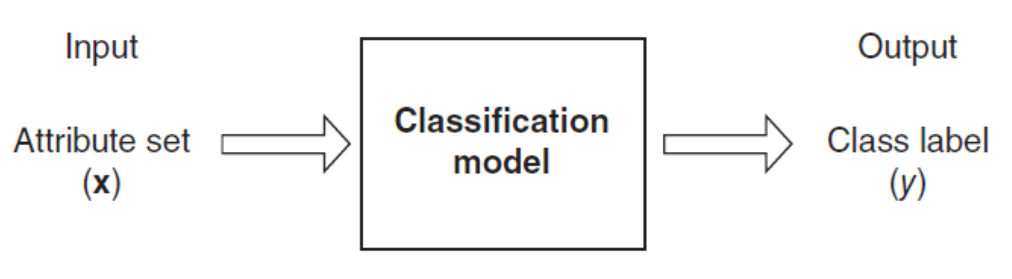
\includegraphics[scale = 0.6]{Images/classification.png}
    \caption{A schematic illustration of a classification task by Tan et al. \cite[p.~134]{DBLP:books/aw/TanSKK2019}.}
    \label{fig:classifiation}
\end{figure}


%\TODO{maybe difference opinion, sentiment, subjectivity?}
%According to Pang and Lee sentiment analysis "deals with the computational treatment of [...] opinion, sentiment, and subjectivity in text" \cite[p.~5]{DBLP:journals/ftir/PangL07}.  Pang and Lee suggest several applications for sentiment analysis, such as review-related websites, in addition to existing technologies such as recommendation systems, as well as business and government intelligence \cite[p.~8]{DBLP:journals/ftir/PangL07}.

\section{Sentiment Analysis}


\subsection{Definition}


Liu defines sentiment analysis, also known as opinion mining, as "the field of study that analyzes people's opinions, sentiments, appraisals, attitudes, and emotions toward entities and their attributes expressed in written text" \cite[p.~1]{liu_2015}. He states that entities include "products, services, organizations, individuals, events, issues, or topics" \cite[p.~1]{liu_2015}. He further analyzes the difference between sentiment and opinion, citing the Merriam-Webster dictionary. There, "sentiment is defined as an attitude, thought, or judgment prompted by feeling, while opinion is defined as a view, judgment, or appraisal formed in the mind" \cite[p.~2]{liu_2015}. Considering this definition, a subtle difference can be seen, where sentiment tends to be viewed more as a feeling, while an opinion is a more concrete view. Although this difference exists, sentiment analysis and opinion mining are still used interchangeably to refer to the same field. Liu defines the term opinion as an encompassing term that includes not only sentiment, but also additional information, such as the opinion holder. A more formal definition of an opinion by Liu can be seen in Equation \eqref{eq:opinion}:
\begin{equation}
    opinion = (e, a, s, h, t),
    \label{eq:opinion}
\end{equation}
where $e$ denotes an entity, $a$ is the target aspect of $e$, $s$ represents the sentiment, $h$ describes the opinion holder, and $t$ the time when the opinion was published \cite{liu_2015}. To further illustrate the difference, the example sentence "I like the display of my Dell laptop", published on 07.05.2022 by Max Mustermann is considered. Here, the entity $e$ is the target of the opinion, the Dell laptop, while $a$ is the specific attribute of the laptop that the sentiment relates to, the display. The sentiment $s$ is qualified as positive, the opinion holder $h$ is Max Mustermann, and the time $t$ is 07.05.2022, resulting in the quintuple (Dell laptop, Display, Positive, Max Mustermann, 07.05.2022). If an opinion does not target a specific aspect, but rather the entire entity, the aspect is defined as "GENERAL" \cite{liu_2015}. 


Liu identifies three different levels of analysis. The document level classifies an entire document as positive or negative, while assuming that it relates to a single entity, such as a product review. The next level is the sentence level, which determines the sentiment of each sentence, including neutral if it does not contain an opinion. The aspect level includes the entity and aspect with which an opinion is concerned \cite{liu_2015}.

Most research identifies two tasks in sentiment analysis. Pang and Lee, for example, differentiate between detection of polarity and detection of subjectivity. The most common form of polarity detection is called sentiment polarity classification, which aims to label an opinionated document as either positive or negative. Polarity may also be viewed as a multiclass problem, where the degrees of positivity are considered, as well as the neutral class, which Pang and Lee describe as the middle ground between positive and negative. Subjectivity detection, on the other hand, seeks to determine whether a given text contains a subjective opinion or is objective. Pang and Lee note that they make a distinction between neutral and objective, the latter being a lack of opinion \cite{DBLP:journals/ftir/PangL07}. Other researchers such as Liu define neutral as being the lack of opinion, noting that an objective sentence may still imply sentiment \cite{liu_2015}. Especially in human-coded data sets, the difference between objective and neutral is often problematic. For example, Nakov et al. instructed their coders to determine whether a sentence is objective, positive, negative, or neutral. Once Nakov et al. used this data set in their sentence polarity task, they combined sentences with an objective and neutral score to one class, as the coders often confused the two classes \cite{nakov-etal-2013-semeval}.

\begin{figure}
    \centering
    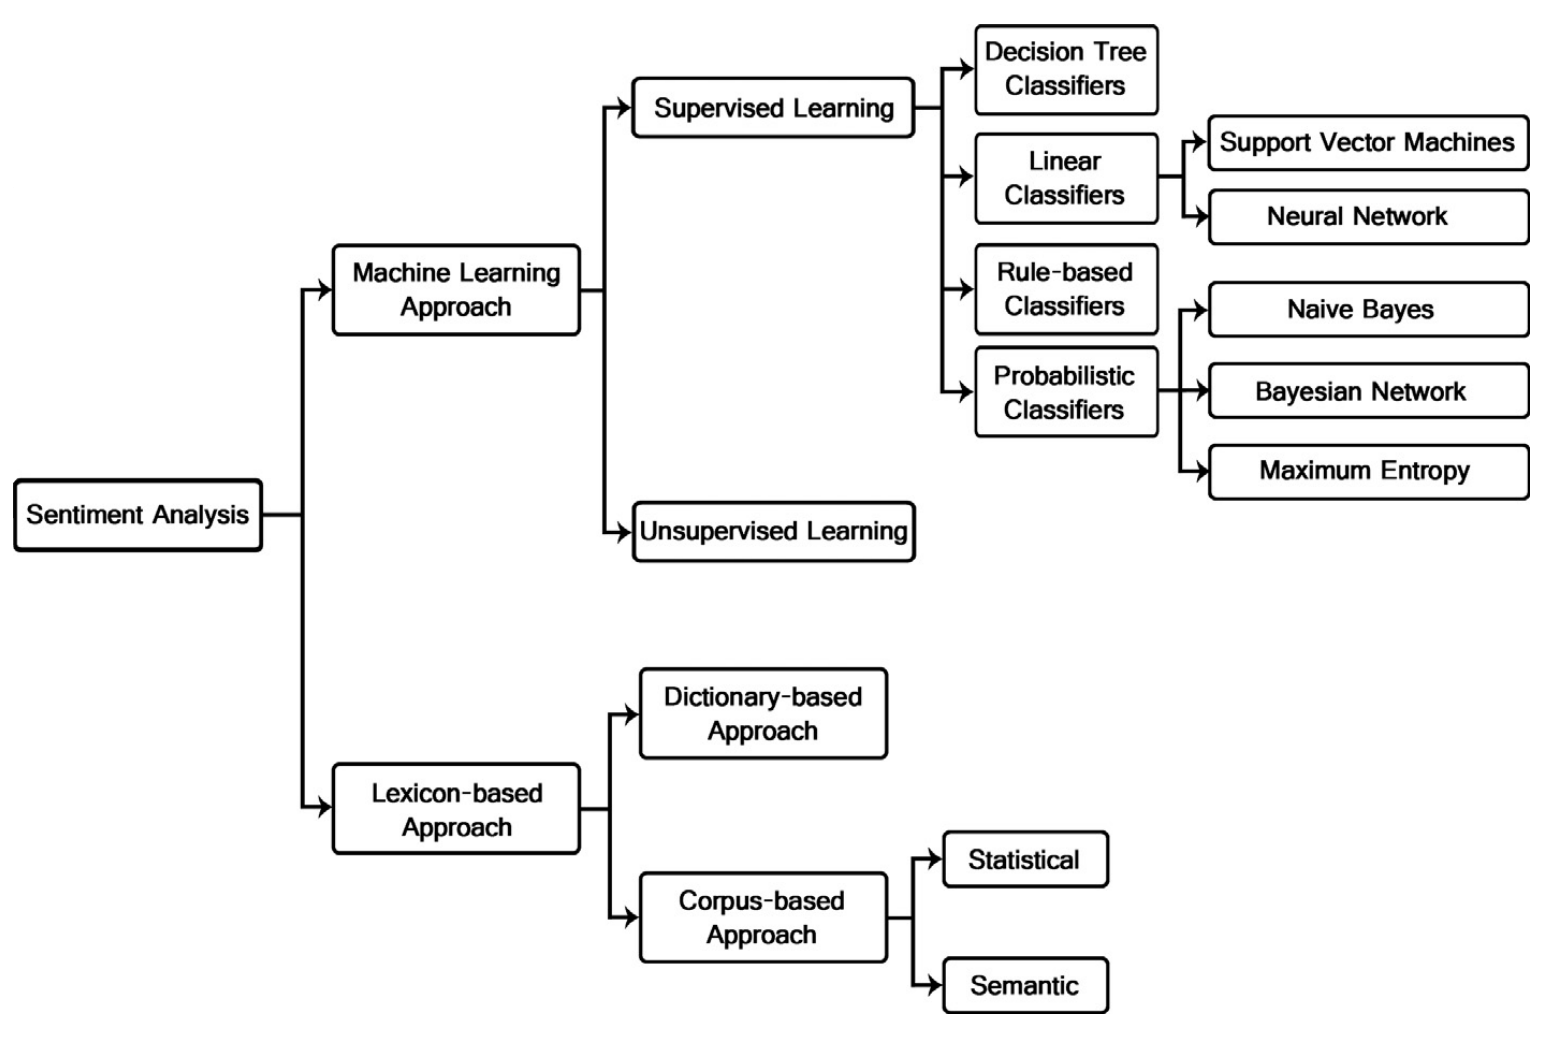
\includegraphics[scale=0.3]{Images/classification_techniques.png}
    \caption{Sentiment classification techniques by Medhat et al. \cite[p.~1095]{MEDHAT20141093}.}
    \label{fig:classifiers}
\end{figure}

\subsection{Approaches}
For polarity classification, Medhat et al. divide approaches into three categories, machine learning, lexicon-based, and hybrid \cite{MEDHAT20141093}. Giachanou and Crestani identify a fourth technique, graph-based methods \cite{DBLP:journals/csur/GiachanouC16}, which are not considered in this thesis. The most important classifiers are shown in Figure \ref{fig:classifiers} and are outlined in the following sections. 

\subsubsection{Machine learning classifiers}
\label{sub:fund_mach}
In general, the machine learning approach treats sentiment analysis as a text classification problem, employing training data to classify unknown instances. Supervised machine learning utilizes labeled training documents together with classifiers such as Naive Bayes. Because it can be difficult to generate a large number of labeled training data, unsupervised approaches are also applied, which rely solely on unlabeled data \cite{MEDHAT20141093}. The supervised methods are further subdivided. According to Tan et al., probabilistic classifiers, such as Naive Bayes and Logistic Regression, "make use of probability theory to represent the relationship between attributes and class labels" \cite[p.~414]{DBLP:books/aw/TanSKK2019}. Linear classifiers, on the other hand, try to find a hyperplane to separate instances from different classes \cite{MEDHAT20141093}. Decision Tree Classifiers, such as Random Forest, use attribute values to divide data into a tree structure. Finally, rule-based classifiers utilize a set of rules to classify an instance \cite{DBLP:books/aw/TanSKK2019}.

Feature selection is one of the essential parts of machine learning, as a classifier relies on the provided attributes. Giachanou and Crestani identify several different possible features for Twitter sentiment analysis: (1) Semantic features, for example, sentiment words and negations, which are extracted using lexicons; (2) Syntactic features, such as the presence of a word or term; (3) Stylistic features, which include emoticons and punctuation; and (4) Twitter-specific features, for example, hashtags or the number of replies \cite{DBLP:journals/csur/GiachanouC16}. For syntactic features, approaches differentiate on how to implement them. Some approaches look at each word of a tweet separately, which is called the unigram model, while others combine two (bigram model) or more words (n-gram model) as a combined feature.

\subsubsection{Lexicon-based methods}
\label{sub:fund_lex}
As stated previously, the lexicon-based approach requires a sentiment lexicon to identify sentiment words and their polarities. In addition, modifiers such as intensifiers and negations can be included to adjust sentiment values \cite{liu_2015}. There are three different methods for building a sentiment lexicon, which are outlined by Medhat et al. There is the manual collection of words, which is very time-intensive. A dictionary-based approach, which starts with a small list of sentiment words, can also be used. It subsequently searches dictionaries for synonyms and antonyms of the sentiment words, maintaining the orientations for synonyms and reversing them for antonyms. The found words are then added to the list and considered in the next iteration. The corpus-based approach utilizes context-specific orientations along with a list of opinion words to find other opinion words in a large corpus. It is based on sentiment consistency, which assumes that adjectives conjoined by "and" have the same polarity, while "but" would signify opposing polarities. This approach can be further subdivided into statistical approaches, which find words using statistics, and semantic approaches, which utilize semantic relationships \cite{MEDHAT20141093}.

\subsubsection{Hybrid methods}

Hybrid methods combine lexicon-based and machine learning methods to balance their disadvantages. Lexicon-based methods are inherently static, as they depend on a set list of words. If a tweet contains words that do not appear in the lexicon, the lexicon-based method cannot classify it. On the other hand, a machine-learning method requires a large amount of labeled training data that is not easy to obtain manually. Hybrid approaches include using the lexicon-based score as an additional feature for the machine learning classifier, or employing multiple different classifiers by, for example, voting on the result \cite{DBLP:journals/csur/GiachanouC16}.


\section{Twitter}
Twitter is a microblogging service, which allows users to send messages, so-called "tweets", containing text, media, and URLs \cite{DBLP:journals/csur/GiachanouC16}. It is one of the largest social media platforms with 330 million monthly users in the first quarter of 2019, who posted 500 million messages daily \cite{twitter:users}. According to Pew Research Center, 23\% of U.S adults used Twitter, and the platform also had the second lowest age gap among the most popular social media platforms \cite{pew:socialmedia}. The length of a tweet was originally restricted to 140 characters until the company expanded the size to 280 characters in 2017 \cite{twitter:characters}. Due to this, Twitter offers a large number of short messages on varying topics made by varying user groups. 

Figure \ref{fig:example_tweet} shows an example of a tweet made by NASA for the Phoenix mission. An account is identified by its unique username, in the example tweet "@MarsPhoenix", and a tweet is identified by its unique tweet ID. The tweet ID can be gathered from the URL of a tweet; the example tweet was assigned the ID "839088619". There are several ways to interact with a tweet. A tweet can be (1) replied to, (2) retweeted, which shares the tweet to a user's profile, (3) quoted, which adds a comment to the retweet, or (4) liked. Other users can also be mentioned in a tweet, with their username being identified by the "@" character. 

\begin{figure}
    \centering
    
\includegraphics[scale=0.3]{Images/twitter_image.png}
    \caption{Picture of a tweet made by the @MarsPhoenix account \cite{twitter:tweet}.}
    \label{fig:example_tweet}
\end{figure}

Twitter's characteristics lead to challenges when applied to sentiment analysis, which are outlined by Giachanou and Crestani. The short length of tweets differs from other domains often used in sentiment analysis, such as movie reviews, which are much longer. After analyzing this topic, Bermingham and Smeaton concluded that classification of sentiment on microblogs is easier than classifying longer documents \cite{microblogs}.

The informal nature of Twitter and its length restrictions frequently lead to abbreviations, slang, and misspellings, which must be considered. Especially emphatic lengthening, which refers to the usage of repeated letters in order to amplify a word, for example, "gooood", is very common in Twitter \cite{DBLP:journals/csur/GiachanouC16}. These characteristics lead to data sparsity, since many terms appear infrequently over an entire corpus of tweets \cite{DBLP:journals/csur/GiachanouC16}. Tan et al. define that for sparse data, most attribute values of a data object are 0 \cite{DBLP:books/aw/TanSKK2019}. Applied to sentiment analysis, the vast majority of observed words, and thus features, do not appear in a tweet. Saif et al. observed that 93\% of the words in their Twitter corpus occurred less than 10 times, compared to 78\% in movie review data \cite{data_sparsity}. 

Twitter offers two APIs to retrieve and analyze Twitter data, REST and streaming \cite{DBLP:journals/csur/GiachanouC16}. There currently are three different access levels, which provide different rates and limits. The elevated level, for example, allows the retrieval of up to 2 million tweets per month \cite{twitter:about}. The REST API provides a short-lived connection, through which several functionalities can be accessed, such as the lookup, creation, and deletion of tweets. Most importantly, it can also be used to search for tweets. Twitter differentiates between recent search, which provides access to public tweets posted in the last week, and full-archive search, which enables access to every tweet ever made. For full-archive search, academic research access is needed. Tweets can be filtered according to parameters such as language, content, and type (e.g. retweet) \cite{twitter:search}. 

The streaming API allows developers to access a real-time stream of tweets, which can be filtered using rules \cite{twitter:stream}. All information is returned in a JSON format, which can be easily parsed by many programming languages. Thus, the Twitter API provides a great method to collect large amounts of tweets \cite{DBLP:journals/csur/GiachanouC16}.




